%!TEX encoding = UTF-8 Unicode

\documentclass[landscape]{book}
\usepackage[a3paper]{geometry}

\usepackage{verbatim}

\usepackage{hyperref}

\usepackage{tikz}

\usetikzlibrary{
  arrows,
  shapes.misc,% wg. rounded rectangle
  shapes.arrows,%
  matrix,%
  scopes,%
  shadows%
}

\tikzset{
  nonterminal/.style={
    % The shape:
    rectangle,
    % The size:
    minimum size=6mm,
    % The border:
    very thick,
    draw=red!50!black!50,         % 50% red and 50% black,
                                  % and that mixed with 50% white
    % The filling:
    top color=white,              % a shading that is white at the top...
    bottom color=red!50!black!20, % and something else at the bottom
    % Font
    font=\itshape\small
  },
  terminal/.style={
    % The shape:
    rounded rectangle,
    minimum size=6mm,
    % The rest
    very thick,draw=black!50,
    top color=white,bottom color=black!20,
    font=\ttfamily\small
  },
  firstPoint/.style={circle,>=stealth',thick,draw=black!50},
  point/.style={coordinate,>=stealth',thick,draw=black!50},
  tip/.style={->,shorten >=0.007pt},
  lastPoint/.style={rectangle,>=stealth',thick,draw=black!50},
  every join/.style={rounded corners}
}

\newcommand\nonTerminalSection[2]{\section{Nonterminal \texttt{#1}}\label{nt:#2}}
\newcommand\ruleSubsection[3]{\subsection{Component \texttt{#1}, in file \texttt{#2}, line #3}}
\newcommand\ruleMatrixColumnSeparation{3mm}
\newcommand\ruleMatrixRowSeparation{3mm}
\newcommand\nonTerminalSymbol[2]{\hyperref[nt:#2]{#1}}
\newcommand\startSymbol[2]{The start symbol is \hyperref[nt:#2]{#1}.}

\newcommand\nonTerminalSummaryStart{This is the alphabetical list of non terminal : }
\newcommand\nonTerminalSummary[2]{\hyperref[nt:#2]{#1}}
\newcommand\nonTerminalSummarySeparator{, }
\newcommand\nonTerminalSummaryEnd{.\\}

\begin{document}

\title{\Huge{Grammar \texttt{arxml\_grammar}}}
\date \today 

\maketitle

\startSymbol{arxml\_start\_symbol}{0}

\nonTerminalSummaryStart \nonTerminalSummary{arxml\_start\_symbol}{0}\nonTerminalSummarySeparator \nonTerminalSummary{element}{2}\nonTerminalSummarySeparator \nonTerminalSummary{element\_list}{1}\nonTerminalSummaryEnd \nonTerminalSection{arxml\_start\_symbol}{0}

\ruleSubsection{arxml\_parser}{arxml\_parser}{31}

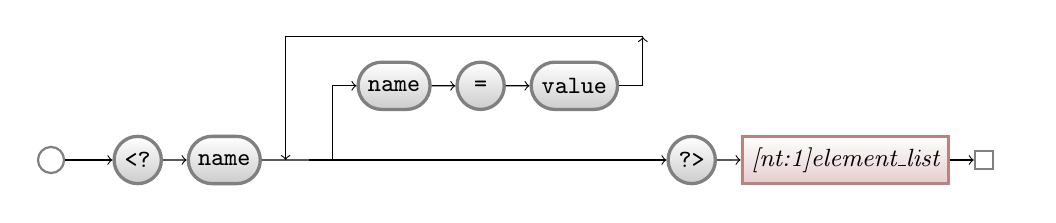
\begin{tikzpicture}
  \matrix[column sep=\ruleMatrixColumnSeparation, row sep=\ruleMatrixRowSeparation] {
    & & & & & & & & & & \node (p2-10) [point] {}; & \\
    & & & & & & & \node (p1-7) [terminal] {name}; & \node (p1-8) [terminal] {=}; & \node (p1-9) [terminal] {value}; & \\
    \node (P0start) [firstPoint] {}; & & \node (p0-2) [terminal] {<?}; & \node (p0-3) [terminal] {name}; & \node (p0-4) [point] {}; & \node (p0-5) [point] {}; & \node (p0-6) [point] {}; & & & & & \node (p0-11) [terminal] {?>}; & \node (p0-12) [nonterminal] {\nonTerminalSymbol{element\_list}{1}}; & \node (p0-13) [lastPoint] {}; & \\
  };
  \draw[->] (P0start) -- (p0-2) ;
  \draw[->] (p0-2) -- (p0-3) ;
  \draw (p0-3) -- (p0-5) ;
  \draw[->] (p0-6) |- (p1-7) ;
  \draw[->] (p1-7) -- (p1-8) ;
  \draw[->] (p1-8) -- (p1-9) ;
  \draw[->] (p2-10) -| (p0-4) ;
  \draw[->] (p1-9) -| (p2-10) ;
  \draw[->] (p0-5) -- (p0-11) ;
  \draw[->] (p0-11) -- (p0-12) ;
  \draw[->] (p0-12) -- (p0-13) ;
\end{tikzpicture}

\nonTerminalSection{element}{2}

\ruleSubsection{arxml\_parser}{arxml\_parser}{205}

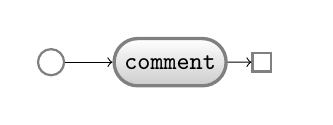
\begin{tikzpicture}
  \matrix[column sep=\ruleMatrixColumnSeparation, row sep=\ruleMatrixRowSeparation] {
    \node (P0start) [firstPoint] {}; & & \node (p0-2) [terminal] {comment}; & \node (p0-3) [lastPoint] {}; & \\
  };
  \draw[->] (P0start) -- (p0-2) ;
  \draw[->] (p0-2) -- (p0-3) ;
\end{tikzpicture}

\ruleSubsection{arxml\_parser}{arxml\_parser}{218}

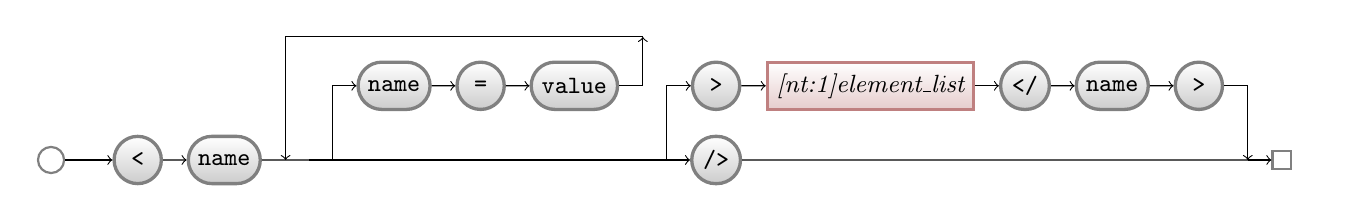
\begin{tikzpicture}
  \matrix[column sep=\ruleMatrixColumnSeparation, row sep=\ruleMatrixRowSeparation] {
    & & & & & & & & & & \node (p2-10) [point] {}; & \\
    & & & & & & & \node (p1-7) [terminal] {name}; & \node (p1-8) [terminal] {=}; & \node (p1-9) [terminal] {value}; & & & \node (p1-12) [terminal] {>}; & \node (p1-13) [nonterminal] {\nonTerminalSymbol{element\_list}{1}}; & \node (p1-14) [terminal] {</}; & \node (p1-15) [terminal] {name}; & \node (p1-16) [terminal] {>}; & \\
    \node (P0start) [firstPoint] {}; & & \node (p0-2) [terminal] {<}; & \node (p0-3) [terminal] {name}; & \node (p0-4) [point] {}; & \node (p0-5) [point] {}; & \node (p0-6) [point] {}; & & & & & \node (p0-11) [point] {}; & \node (p0-12) [terminal] {/>}; & & & & & \node (p0-17) [point] {}; & \node (p0-18) [lastPoint] {}; & \\
  };
  \draw[->] (P0start) -- (p0-2) ;
  \draw[->] (p0-2) -- (p0-3) ;
  \draw (p0-3) -- (p0-5) ;
  \draw[->] (p0-6) |- (p1-7) ;
  \draw[->] (p1-7) -- (p1-8) ;
  \draw[->] (p1-8) -- (p1-9) ;
  \draw[->] (p2-10) -| (p0-4) ;
  \draw[->] (p1-9) -| (p2-10) ;
  \draw[->] (p0-5) -- (p0-12) ;
  \draw[->] (p0-11) |- (p1-12) ;
  \draw[->] (p1-12) -- (p1-13) ;
  \draw[->] (p1-13) -- (p1-14) ;
  \draw[->] (p1-14) -- (p1-15) ;
  \draw[->] (p1-15) -- (p1-16) ;
  \draw (p0-12) -- (p0-17) ;
  \draw[->] (p1-16) -| (p0-17) ;
  \draw[->] (p0-17) -- (p0-18) ;
\end{tikzpicture}

\nonTerminalSection{element\_list}{1}

\ruleSubsection{arxml\_parser}{arxml\_parser}{185}

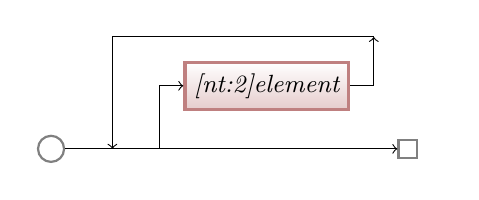
\begin{tikzpicture}
  \matrix[column sep=\ruleMatrixColumnSeparation, row sep=\ruleMatrixRowSeparation] {
    & & & & & & \node (p2-6) [point] {}; & \\
    & & & & & \node (p1-5) [nonterminal] {\nonTerminalSymbol{element}{2}}; & \\
    \node (P0start) [firstPoint] {}; & & \node (p0-2) [point] {}; & \node (p0-3) [point] {}; & \node (p0-4) [point] {}; & & & \node (p0-7) [lastPoint] {}; & \\
  };
  \draw (P0start) -- (p0-3) ;
  \draw[->] (p0-4) |- (p1-5) ;
  \draw[->] (p2-6) -| (p0-2) ;
  \draw[->] (p1-5) -| (p2-6) ;
  \draw[->] (p0-3) -- (p0-7) ;
\end{tikzpicture}



\end{document}
